The Cox-Ingersoll-Ross model (CIR) is a mathematical formula used
to model interest rate movements.
It was introduced by John Carrington Cox, Jonathan Edwards Ingersoll
and Stephen Alan Ross in 1985.
An interest rate model is, essentially, a probabilistic description of
how interest rates can change over time.

Interest rates have properties such as positivity, boundedness,
and return to equilibrium which make them behave differently from stock and
asset prices.
CIR model describes interest movements as driven by a sole source of market
risk.
It is used as a method to forecast interest rates and is based on a
stochastic differential equation.

CIR is a mean reverting process, the square root element($\sqrt{r_t}$) does
not allow for negative rates and the model assumes mean reversion towards a
long-term normal interest rate level.


\subsection{SDE}
The CIR model describes the dynamics of the interest rate r(t) as a
solution of the following stochastic differential equation (SDE):
\begin{equation}
	\begin{cases}
		d r(t)=\kappa(\theta-r(t)) d t+\sigma \sqrt{r(t)} d W(t) \\
		r(0)=r_{0}
	\end{cases}
	\label{eq:sde-cir}
\end{equation}
where,
\begin{enumerate}
	\item $\kappa$ mean reversion coefficient
	\item $\theta$ long term mean
	\item $\sigma$ volatility coefficient
\end{enumerate}
In this model, the stochastic term $\sigma \sqrt{r(t)} d W(t)$ has a
standard deviation proportion to the square root of the current rate.
This implies that as the rate increase, its standard deviation increase and
as it falls and approach zero, the stochastic term also approach zero.


\subsection{Assumptions}
There are three assumptions in this model,
\begin{enumerate}
	\item The change in the interest rate over time is described by a
	single state variable $r$.
	\item The means and variances of the rates of return in the
	processes are proportional to $r$, which means that they won’t
	dominate the portfolio decision for large values of $r$.
	\item The development of the state variable $r$ follows
	the equation~\ref{eq:sde-cir}.
\end{enumerate}


\subsection{Modelling the formula}

For modelling the CIR formula, we need to find the
parameters of the formula $\theta$, $\kappa$ etc.
based on the real world data, for this we use Method of Moments
technique for parameter estimation.

This technique has been thoroughly explained in the following
Heston model Section, intuitively one may understand that this
technique is based on equating the $n^{th}$ theoretical moment of a
random variable with corresponding sample moment, and solving
these equations to find the required parameters.

So, in the following subsections we derive some results towards finding a
general equation for the theoretical moments of $r$.



\subsection{Exact Solution}
The Integral form of the above stochastic differential
equation~\ref{eq:sde-cir} is:
\begin{equation}
	r(t) = \theta + (r_0 - \theta)e^{-\kappa t} + \sigma e^{\kappa t}
	\int_{0}^{t}e^{\kappa s}\sqrt{r(s)}dW(s)
	\label{eq:closed-cir}
\end{equation}
\textit{Proof :}

The equation~\ref{eq:sde-cir} changes to the following form
\begin{equation}
	dr(t)+\kappa r(t)dt=\kappa \theta dt+\sigma \sqrt{r(t)}dW(t)
	\label{eq:eq-1}
\end{equation}
Multiplying both sides of the relation~\ref{eq:eq-1} by
$e^{\kappa t}$ results in
\begin{align}
	e^{\kappa t} d r(t)+\kappa e^{\kappa t} r(t) d t &=\kappa
		\theta e^{\kappa t} d t+\sigma e^{\kappa t} \sqrt{r(t)} d W(t) \\
	d\left(e^{\kappa t} r(t)\right) &=\kappa \theta e^{\kappa t}
		d t+\sigma e^{\kappa t} \sqrt{r(t)} d W(t)
		\label{eq-2}
\end{align}
Now, integrating both sides of the relation~\ref{eq-2} on $[0, t]$ gives us
\begin{equation}
	e^{\kappa t} r(t)-r_{0}=\kappa \theta \int_{0}^{t} e^{\kappa s}
	d s+\sigma \int_{0}^{t} e^{\kappa s} \sqrt{r(s)} d W(s)
	\label{eq:eq-3}
\end{equation}

Consequently, the relation~\ref{eq:eq-3} is derived.

According to the above result, the CIR model has no general explicit solution.
However, its mean and variance can be calculated explicitly.


\subsection{Expectation and Variance}
The expectation and variance of $r_t \coloneqq r(t)$ are given by
\begin{align}
	\begin{cases}
		\Exp{r_t} = e^{-\kappa t} r_0  + \theta \brak{1 - e^{-\kappa t}} \\
		\Var{r_t} = \frac{\sigma^2}{\kappa} r_0
			\brak{e^{-\kappa t} - e^{-2\kappa t}} +
			\frac{\theta\sigma^2}{2\kappa} \brak{1 - e^{-\kappa t}}^2
	\end{cases}
\end{align}

\textit{Proof.}
\begin{align*}
	\Exp{r_t} &= \Exp{e^{-\kappa t} r_0 + \theta
		\brak{1 - e^{-\kappa t}} + \sigma
		\int_0^t e^{\kappa s} \sqrt{r_s} dW_s} \\
	&= e^{-\kappa t} r_0 + \theta\brak{1 - e^{-\kappa t}} +
		\Exp{\sigma \int_0^t e^{\kappa s} \sqrt{r_s} dW_s} \\
		\therefore \Exp{r_t} &= e^{-\kappa t} r_0 +
		\theta \brak{1 - e^{-\kappa t}} \numberthis \label{eq:exp-cir}
\end{align*}

\begin{align*}
	\Var{r_t} &= \Exp{r_t^2} - \Exp{r_t}^2 \\
	&= \Exp{\brak{e^{-\kappa t} r_0 + \theta
		\brak{1 - e^{-\kappa t}} + \sigma e^{-\kappa t}
		\int_0^t e^{\kappa s} \sqrt{r_s} dW_s}^2} \\
		& \quad \quad \quad - \Exp{r_t}^2 \\
	&= \Exp{\brak{\Exp{r_t} + \sigma e^{-\kappa t}
		\int_0^t e^{\kappa s} \sqrt{r_s} dW_s}^2}
		- \Exp{r_t}^2 \\
	&= 2\Exp{\Exp{r_t} \sigma e^{-\kappa t}
		\int_0^t e^{\kappa s} \sqrt{r_s} dW_s} \\
		& \quad \quad \quad
		+ \Exp{\brak{\sigma e^{-\kappa t} \int_0^t e^{\kappa s}
		\sqrt{r_s} dW_s}^2} \\
	&= 2\ \Exp{r_t} e^{-\kappa t} \cdot 0 +
		\Exp{\brak{\sigma e^{-\kappa t} \int_0^t e^{\kappa s}
		\sqrt{r_s} dW_s}^2} \\
	&= \Exp{\sigma^2 e^{-2\kappa t} \int_0^t e^{2\kappa s} r_s ds}
		\quad (\text{Iso Isometry}) \\
	&= \sigma^2 e^{-2\kappa t}
		\int_0^t e^{2\kappa s} \Exp{r_s} ds \\
	&= \sigma^2 e^{-2\kappa t}
		\int_0^t e^{2\kappa s} \brak{e^{-\kappa s} r_0 +
		\theta \brak{1 - e^{-\kappa s}}} ds \\
	&= \frac{\sigma^2}{\kappa} e^{-2\kappa t} r_0
		\brak{e^{\kappa s} - 1}
		+ \theta\sigma^2 e^{-2\kappa t}
		\int_0^t \brak{e^{2\kappa s} - e^{\kappa s}} ds \\
	&= \frac{\sigma^2}{\kappa} r_0
		\brak{e^{-\kappa t} - e^{-2\kappa t}} +
		\frac{\theta\sigma^2}{2\kappa} \brak{1 - e^{-\kappa t}}^2
		\numberthis \label{eq:var-cir}
\end{align*}


\subsection{\( 3^{rd} \) Moment of \( r_t \)}
\[ \Exp{r_t^3} = \Exp{\brak{A_t + B_t I_t}^3} \] where
\( A_t = e^{-\kappa t} r_0 + \theta \brak{1 - e^{-\kappa t}} \quad \)
\( B_t = \sigma e^{-\kappa t} \) and \\
\( \displaystyle I_t = \int_0^t e^{\kappa s} \sqrt{r_s} dW_s \quad \)
\begin{align}
	\Exp{r_t^3} &= \Exp{\brak{A_t + B_t I_t}^3} \\
	&= A_t^3 + 3A_t^2 B_t\Exp{I_t} + 3A_t B_t^2\Exp{I_t^2} \nonumber \\
	& \quad \quad + B_t^3\Exp{I_t^3} \\
	&= A_t^3 + 3A_t B_t^2\Exp{I_t^2} \\
	&= A_t \brak{A_t^2 + B_t^2 \int_0^t e^{2\kappa s} \Exp{r_s} ds } \\
	&= \Exp{r_t} \brak{\Exp{r_t}^2 + \Var{r_t}}
\end{align}


\subsection{Parameter Estimation}
We equate the moments obtained from method of moments and sample moments to
estimate the parameters $\kappa$,$\theta$ and $\sigma$.

\subsection{CIR-path}

\begin{figure}[!ht]
	\centering
	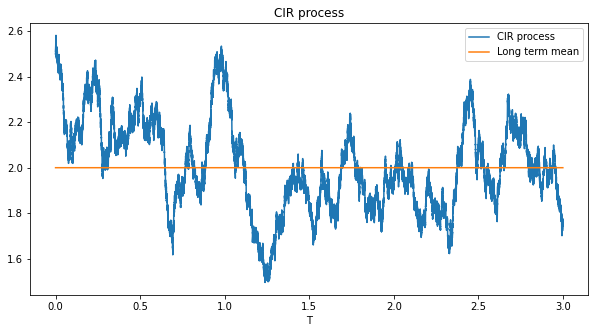
\includegraphics[width=\textwidth/2]{figs/CIR}
	\caption{Caption}
	\label{fig:cir-process}
\end{figure}
